\section{Latar Belakang AES}

Pada Bab~\ref{chap:des} telah ditunjukkan bahwa kelemahan terpenting DES bukanlah
struktur internalnya, melainkan panjang kuncinya. Dengan kunci efektif hanya 56 bit,
seluruh ruang kunci berisi $2^{56} = 72.057.594.037.927.936$ kemungkinan, dan ruang
sebesar itu sudah dapat ditelusuri habis oleh perkakas khusus maupun jaringan komputer
umum pada akhir dekade 1990-an. Bila pada tahun 1977 penelusuran menyeluruh memerlukan
waktu ribuan tahun, pada tahun 1998 \textit{Electronic Frontier Foundation} membangun
mesin \textit{Deep Crack} senilai \$250.000 yang menyelesaikannya dalam 56 jam
\citep{eff1998}. Artinya, DES berhenti menjadi sandaran yang memadai jauh sebelum masa
pakainya berakhir.

Kerusakan seperti itu tidak dapat diperbaiki dengan menambal DES, misalnya dengan
memperpanjang kuncinya atau menambah putarannya; yang dibutuhkan adalah standar
enkripsi blok yang sepenuhnya baru. Kesulitan utamanya bukan teknis melainkan
sosial: bagaimana sebuah standar baru dapat dipercaya oleh seluruh dunia, mengingat
DES sendiri sejak awal dicurigai karena proses perancangannya tertutup dan melibatkan
campur tangan badan keamanan. \textit{National Institute of Standards and Technology}
(NIST) menjawab kesulitan itu dengan cara yang berlawanan: menyelenggarakan kompetisi
terbuka.

\subsection{Kompetisi Terbuka NIST}

NIST mengumumkan sayembara untuk \textit{Advanced Encryption Standard} (AES) pada
September 1997 dan merumuskan lima persyaratan yang harus dipenuhi setiap calon.
Persyaratan itu penting untuk dipahami karena sekaligus menjadi garis besar
karakteristik AES yang kita pelajari hari ini:

\begin{enumerate}
    \item \textbf{Jenis algoritma.} Calon harus berupa cipher blok simetri, yaitu
    algoritma dengan satu kunci yang sama untuk enkripsi dan dekripsi.
    \item \textbf{Rancangan publik.} Seluruh rancangan harus terbuka dan dapat
    diperiksa siapa pun; tidak boleh ada bagian yang dirahasiakan.
    \item \textbf{Panjang kunci fleksibel.} Harus mendukung kunci 128, 192, dan 256 bit.
    \item \textbf{Ukuran blok tetap.} Blok yang dienkripsi berukuran 128 bit.
    \item \textbf{Efisiensi.} Harus dapat diimplementasikan dengan baik, baik sebagai
    perangkat lunak maupun perangkat keras.
\end{enumerate}

Dari 21 naskah yang masuk, 15 dinyatakan memenuhi syarat dan masuk babak pertama
(Augustus 1998). Babak kedua (Agustus 1999) menyisakan lima finalis, yang
perolehan suaranya tercantum pada Tabel~\ref{tab:finalis-aes}. Penilaian tidak hanya
menimbang keamanan, tetapi juga kecepatan pada berbagai platform, kebutuhan memori,
kesederhanaan rancangan, dan keluwesan implementasi.

\begin{table}[htbp]
\centering
\caption{Lima finalis sayembara AES beserta perancang dan perolehan suaranya}
\label{tab:finalis-aes}
\small
\begin{tabularx}{\linewidth}{@{}l l >{\raggedright\arraybackslash}X c@{}}
\hline
\textbf{Algoritma} & \textbf{Perancang} & \textbf{Karakteristik rancangan} & \textbf{Suara} \\
\hline
Rijndael  & Rijmen \& Daemen (Belgia)      & SPN berorientasi byte, kunci dan blok dapat dipilih & 86 \\
Serpent   & Anderson, Biham, Knudsen       & SPN 32 putaran, bit-slice, margin keamanan besar & 59 \\
Twofish   & Schneier dkk.\ (Amerika)       & Jaringan Feistel 16 putaran, S-box bergantung kunci & 31 \\
RC6       & Laboratorium RSA (Amerika)     & Turunan RC5, rotasi bergantung data & 23 \\
MARS      & IBM (Amerika)                  & Campuran Feistel dan SPN, putaran heterogen & 13 \\
\hline
\end{tabularx}
\sumber{Munir, \textit{IF4020 Kriptografi}, ITB.}
\end{table}

Pada Oktober 2000 NIST mengumumkan pemenangnya, yaitu \textbf{Rijndael}, rancangan
Joan Daemen dan Vincent Rijmen dari Belgia (Gambar~\ref{fig:perancang-aes}). Nama itu
dibaca \textit{rhine-doll}, gabungan nama kedua perancangnya. Pada November 2001
pemenang itu dibakukan sebagai \textbf{FIPS PUB 197} \citep{fips197}, dan sejak saat
itulah nama resminya menjadi AES, sedangkan ``Rijndael'' tetap dipakai untuk merujuk
keluarga algoritma aslinya.

\begin{figure}[htbp]
    \centering
    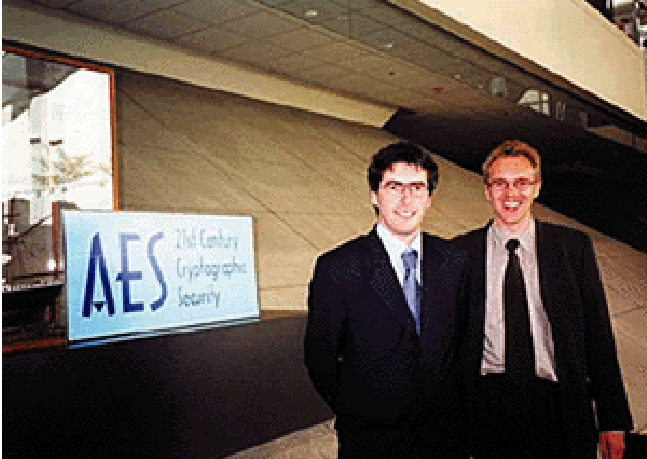
\includegraphics[width=0.62\linewidth]{figures/perancang-aes.png}
    \caption{Joan Daemen dan Vincent Rijmen, perancang Rijndael yang dibakukan menjadi AES}
    \label{fig:perancang-aes}
    \sumber{Munir, \textit{IF4020 Kriptografi}, ITB.}
\end{figure}

\subsection{Rijndael dan AES: Hubungan Keduanya}

Salah satu kekeliruan yang sering muncul adalah menganggap Rijndael dan AES sebagai
dua nama bagi barang yang sama persis. Keduanya memang berbagi algoritma yang sama,
tetapi cakupan parameternya tidak sama. Rijndael adalah sebuah \textit{keluarga}
algoritma dengan dua parameter bebas:

\begin{itemize}
    \item ukuran blok $N_b$ kelipatan 32 bit dari 128 sampai 256 bit, dan
    \item panjang kunci $N_k$ kelipatan 32 bit dari 128 sampai 256 bit.
\end{itemize}

AES hanyalah satu irisan dari keluarga itu, yaitu irisan dengan $N_b = 128$ bit
tetap. Karena itu Rijndael dengan blok 192 bit atau 224 bit bukanlah AES, sedangkan
AES-128, AES-192, dan AES-256 seluruhnya adalah anggota keluarga Rijndael. Nama
belakang pada sebutan ``AES-128'' menunjuk pada \emph{panjang kunci}, bukan pada
jumlah putaran: AES-128 memang berputaran 10, tetapi angka 128 itu mula-mula berarti
128 bit kunci.

Jumlah putaran $N_r$ bukan parameter bebas, melainkan fungsi dari $N_b$ dan $N_k$:
\[
N_r = \max(N_b, N_k) + 6 .
\]
Dengan $N_b = 4$ word (satu word = 32 bit) diperoleh $N_r = 10$ untuk kunci 128 bit,
$N_r = 12$ untuk kunci 192 bit, dan $N_r = 14$ untuk kunci 256 bit. Rumus itu
menunjukkan sebuah pilihan rancangan yang sadar: kunci yang lebih panjang tidak
hanya memperbesar ruang kunci, tetapi juga menambah jumlah putaran sehingga
serangan yang memanfaatkan struktur putaran tetap memerlukan usaha yang sepadan
\citep{daemen2002}. Tabel~\ref{tab:parameter-aes} merangkum ketiga varian AES.

\begin{table}[htbp]
\centering
\caption{Parameter ketiga varian AES}
\label{tab:parameter-aes}
\begin{tabular}{@{}l c c c c c@{}}
\hline
\textbf{Varian} & \textbf{Panjang kunci} & $N_k$ & $N_b$ & $N_r$ & \textbf{Kunci putaran} \\
\hline
AES-128 & 128 bit & 4 word & 4 word & 10 & 11 \\
AES-192 & 192 bit & 6 word & 4 word & 12 & 13 \\
AES-256 & 256 bit & 8 word & 4 word & 14 & 15 \\
\hline
\end{tabular}
\sumber{Munir, \textit{IF4020 Kriptografi}, ITB.}
\end{table}

Perhatikan kolom terakhir. Karena satu kunci putaran berukuran sama dengan satu blok
(128 bit), jumlah kunci putaran selalu $N_r + 1$: satu kunci untuk putaran awal dan
satu kunci untuk setiap putaran sesudahnya. Untuk AES-128 seluruh proses
\textit{KeyExpansion} harus menghasilkan $4(N_r+1) = 44$ word, untuk AES-192
sebanyak $4 \times 13 = 52$ word, dan untuk AES-256 sebanyak $4 \times 15 = 60$ word.
Angka-angka itulah yang menjadi patokan ketika kita memeriksa kebenaran pembangkitan
kunci pada Sub-bab~\ref{sec:key-expansion-aes}.

\subsection{Mengapa AES Dianggap Aman}

Alasan pertama dan paling langsung adalah ukuran ruang kuncinya. Dengan kunci 128 bit
terdapat
\[
2^{128} = 3{,}4 \times 10^{38}
\]
kemungkinan kunci. Untuk memberi gambaran betapa besarnya angka itu, andaikan sebuah
komputer mampu mencoba $10^6$ kunci setiap detik tanpa henti. Penelusuran menyeluruh
memerlukan waktu terburuk
\[
\frac{2^{128}}{10^6 \times 60 \times 60 \times 24 \times 365{,}25}
\approx 1{,}08 \times 10^{25} \text{ tahun},
\]
yaitu sekitar $5{,}4 \times 10^{24}$ tahun bila dirata-ratakan --- masih jauh
melampaui usia alam semesta yang diperkirakan sekitar $1{,}4 \times 10^{10}$ tahun.
Menaikkan laju penyerang menjadi $10^9$ kunci per detik hanya menurunkan angka itu
ke $1{,}08 \times 10^{22}$ tahun (rata-rata $5{,}4 \times 10^{21}$ tahun), yang tetap
tidak berarti secara praktis. Kesimpulannya, AES memang dirancang tahan terhadap
serangan penelusuran kunci menyeluruh (\textit{exhaustive key search attack}).

Akan tetapi, ketahanan terhadap \textit{brute force} hanyalah syarat perlu, bukan
syarat cukup. Kekuatan sesungguhnya justru terletak pada ketiadaan jalan pintas:
tidak boleh ada serangan yang jauh lebih cepat daripada penelusuran menyeluruh.
Sampai saat ini, serangan terbaik terhadap AES penuh masih lebih lambat daripada
penelusuran menyeluruh atas kuncinya, dan serangan yang paling berhasil menyerang
versi yang putarannya dikurangi, bukan versi penuh. Itulah alasan AES masih dipakai
secara luas lebih dari dua dekade setelah dibakukan, jauh melewati target awal
sepuluh tahun.

\subsection{Perbandingan Ringkas dengan DES}

Tabel~\ref{tab:perbandingan-des-aes} memperbandingkan kedua standar secara
berdampingan. Perbandingan ini berguna bukan sekadar sebagai ringkasan, tetapi karena
memperlihatkan dua filosofi rancangan yang berbeda: DES mengulang putaran yang
sederhana berkali-kali dengan bantuan jaringan Feistel, sedangkan AES memakai
sedikit putaran dengan transformasi yang jauh lebih ``padat'' pada setiap putaran.

\begin{table}[htbp]
\centering
\caption{Perbandingan DES dan AES}
\label{tab:perbandingan-des-aes}
\small
\begin{tabularx}{\linewidth}{@{}l >{\raggedright\arraybackslash}X >{\raggedright\arraybackslash}X@{}}
\hline
\textbf{Aspek} & \textbf{DES} & \textbf{AES} \\
\hline
Tahun baku        & FIPS PUB 46, 1977 & FIPS PUB 197, 2001 \\
Ukuran blok       & 64 bit            & 128 bit \\
Panjang kunci     & 56 bit efektif    & 128, 192, atau 256 bit \\
Jumlah putaran    & 16                & 10, 12, atau 14 \\
Struktur          & Jaringan Feistel  & Jaringan substitusi--permutasi \\
Orientasi data    & Bit               & Byte \\
Permutasi         & Tabel $P$ tetap   & ShiftRows (pergeseran baris) \\
Substitusi        & Delapan S-box 6$\to$4 bit & Satu S-box 8$\to$8 bit untuk seluruh byte \\
Dekripsi          & Algoritma sama, kunci dibalik & Algoritma berbeda (transformasi invers) \\
Operasi           & XOR dan permutasi bit & XOR, substitusi byte, aritmetika GF($2^8$) \\
Proses perancangan & Tertutup, disunting NSA & Sayembara terbuka, rancangan publik \\
\hline
\end{tabularx}
\sumber{Munir, \textit{IF4020 Kriptografi}, ITB.}
\end{table}

Baris ``Dekripsi'' pada tabel itu perlu digarisbawahi, karena di situlah perbedaan
paling terasa bagi yang mengimplementasikan. Pada DES, sifat reversibel jaringan
Feistel membuat dekripsi cukup menjalankan enkripsi dengan urutan subkunci terbalik;
fungsi putarannya tidak perlu dibalik sama sekali. Pada AES hal itu tidak berlaku:
kita memerlukan fungsi invers yang benar-benar terpisah, yaitu \textit{InvSubBytes},
\textit{InvShiftRows}, dan \textit{InvMixColumns}. Ketiga fungsi itu dibahas pada
Sub-bab~\ref{sec:mekanisme-aes}, dan justru di situlah letak salah satu kesulitan
utama implementasi AES yang efisien.
